
\chapter{Análisis}

\begin{defn}[Función real de variable real]
Una función real de una variable real es una aplicación definida entre dos conjuntos de números reales tal que a cada elemento del primer conjunto le corresponde un único elemento del segundo conjunto.

$\appl{f}{D\subset\real}{\real}$

\begin{itemize}
	\item $f$: símbolo de la función.
	\item $D(f) = \{x\in\real \tq \exists f(x)\}$
	\item $Rec(f) = \{y\in\real \tq \exists x \in\real f(x)=y\}$
\end{itemize}
\end{defn}


\begin{problem}
Halla el dominio de las siguientes funciones:
\ppart $f(x) = \sqrt{\displaystyle\frac{x^2+5x+4}{x+4}}$ \obs Ojo con simplificar.
\ppart $f(x) = \sqrt{\left(x^2-9\right)}$
\ppart  $f(x) = \log\left(-2x^2+10x-12\right)$
\ppart  $f(x) = \log\left(x^2+1\right)$

\solution


.\vspace{15cm}.


\end{problem}

\paragraph{Funciones de valor absoluto:} (visto en pizarra)


\section{Límites y continuidad}

\subsection{Introducción al concepto de límite}

Visto con Eduardo.

%\begin{itemize}
%	\item Con la hoja excel de MNieves.
%	\item Con el geogebra.
%	\item Ejercicios gráficos de límites (PDF aparte: %"Límites gráficamente")
%\end{itemize}

\subsection{Estudio analítico de límites}

\subsubsection{Propiedades de los límites}

\begin{enumerate}
	\item $\displaystyle\lim_{x\to a} [f(x) \pm g(x)] = \lim_{x\to a} f(x) \pm \lim_{x\to a} g(x)$
	\item $\displaystyle\lim_{x\to a} [f(x) · g(x)] = \lim_{x\to a} f(x) · \lim_{x\to a} g(x)$
	\item $\displaystyle\lim_{x\to a} \frac{f(x)}{g(x)} = \frac{\lim_{x\to a} f(x)}{\lim_{x\to a} g(x)}\quad\text{ si }\displaystyle\lim_{x\to a} g(x) \neq 0$
	\item $\displaystyle\lim_{x\to a} \left(f(x)\right)^p = \left(\lim_{x\to a}f(x)\right)^p \quad \forall p\in\real$
	\item $\displaystyle\lim_{x\to a} \left(f(x)\right)^{g(x)} = \left(\lim_{x\to a}f(x)\right)^{\displaystyle\lim_{x\to a}g(x)} \quad\text{ si }\displaystyle \lim_{x\to a}f(x) \neq 0 \wedge \lim_{x\to a}g(x)\neq 0$
	\item $\displaystyle\lim_{x\to a}\log f(x) = \log\left(\displaystyle\lim_{x\to a}f(x)\right)\quad\text{ si } \lim_{x\to a}f(x) >0 $
\end{enumerate}

\begin{theorem}[Teorema\IS de existencia del límite]
\[\forall a\in \real, \exists \lim_{x\to a}f(x) \dimplies \lim_{x\to a^+} f(x) = \lim_{x\to a^-}f(x)\]
\end{theorem}

\begin{problem}
\begin{itemize}
	\item Página 123, ejercicio 20.
	\item $\displaystyle\lim_{x\to 3} \frac{\log(x-2)}{x-1}$
	\item \label{Analisis::EjemploContinuidad}Sea $f(x) = 
		\begin{cases}
		x+3 & \text{ si } x>0\\
		\frac{2x+3}{x+1}& \text{ si } x\leq 0 
		\end{cases}$ Calcula:
		\subitem $\displaystyle\lim_{x\to 1} f(x)$
		\subitem $\displaystyle\lim_{x\to 0} f(x)$
\end{itemize}
\solution

.\vspace{10cm}.

\end{problem}

\subsubsection{Indeterminaciones}

\begin{itemize}
	\item Racionales: $\rfrac{0}{0},\rfrac{\infty}{\infty},\infty-\infty,0·\infty, \rfrac{k}{0}$ 
	\item Exponenciales $1^{\infty}; 0^0; \infty^0$
\end{itemize}

De estas indeterminaciones, no veremos $0^0; \infty^0$ y de $0·\infty$ nos saldrá alguna en el sigueinte tema.

\subsection{Asíntotas}

\subsubsection{Verticales}

\begin{defn}[Asíntota\IS vertical]

La recta $x=a$ es \textbf{asíntota vertical} de $f(x)\dimplies \displaystyle\begin{cases}\displaystyle\lim_{x\to a^+}f(x) = \pm\infty\\ \text{ó}\\ \displaystyle\lim_{x\to a^+}f(x) = \pm\infty\end{cases}$
\end{defn}

\begin{problem}
Estudia las asíntotas verticales de $f(x) = \frac{x+1}{x^2+x}$ y de $g(x) = \log(x)$
\solution
\end{problem}


\subsubsection{Horizontales}

\begin{defn}[Asíntota\IS horizontal]

La recta $y=b$ es \textbf{asíntota horizontal} de $f(x)$ en $+\infty$ si y solo si $ \displaystyle\lim_{x\to +\infty}f(x) = b$

La recta $y=b$ es \textbf{asíntota horizontal} de $f(x)$ en $-\infty$ si y solo si $ \displaystyle\lim_{x\to -\infty}f(x) = b$

\end{defn}

\subsubsection{Oblicuas}

\begin{defn}[Asíntota\IS oblicua]

La recta $y=mx+n$ es \textbf{asíntota oblicua}

en $+\infty$ de $f(x)\dimplies \displaystyle
\begin{cases}
	\displaystyle\lim_{x\to +\infty}f(x) = \pm\infty\\
 	\displaystyle\lim_{x\to +\infty}\frac{f(x)}{x} = m\in\real\\
 	\displaystyle\lim_{x\to +\infty}(f(x) - m·x) = n
 \end{cases}$

La recta $y=mx+n$ es \textbf{asíntota oblicua} 

en $-\infty$ de $f(x)\dimplies \displaystyle
\begin{cases}
	\displaystyle\lim_{x\to -\infty}f(x) = \pm\infty\\
 	\displaystyle\lim_{x\to -\infty}\frac{f(x)}{x} = m\in\real\\
 	\displaystyle\lim_{x\to -\infty}(f(x) - m·x) = n
 \end{cases}$
\end{defn}

\paragraph{Observación:} Las asíntotas oblicuas y horizontales son mutuamente excluyentes, es decir, no puede haber una asíntota horizontal y una oblicua simultáneamente en un extremo del dominio. Sí podría haber una asíntota horizontal en $+\infty$ y una oblicua en $-\infty$.

\begin{problem}
Estudia el comportamiento asintótico en $\pm\infty$ de las siguientes funciones:
\begin{itemize}
	\item $f(x) = e^x$
	\item $f(x) = \frac{x^2}{3x+1}$
	\item $f(x) = \frac{x^2}{3x^2+1}$
	\item $f(x) = \frac{x^2}{3x^3+1}$
\end{itemize}

\solution

.\vspace{10cm}.

\end{problem}

\paragraph{Observación:} Las funciones racionales tienen el mismo comportamiento asintótico en $+\infty$ que en $-\infty$

\begin{problem}
\textit{Funciones obtenidas de exámenes EvAU}

Estudia el comportamiento asintótico de las siguientes funciones 

$$f_1(x) = \sqrt{\frac{x^2-4}{x^2-1}}$$

$$f_2(x) = \begin{cases}
\frac{x^2+3x+1}{x}&\text{ si }  x\geq -1\\
\frac{2x}{x-1}&\text{ si }  x< -1
\end{cases}
$$

\solution

.\vspace{15cm}.

\end{problem}

\begin{prop}[Indeterminación\IS $1^{\infty}$]
\index{Indeterminación\IS $1^{\infty}$}
\[
\lim_{x\to a}f(x)^{g(x)} \to 1^{\infty} \implies \lim_{x\to a}f(x)^{g(x)} = e^\lambda, \lambda = \lim_{x\to a} \left(g(x)·[f(x)-1]\right)
\]
\end{prop}

\begin{proof}
\begin{align*}
\lim_{x\to a}f(x)^{g(x)} &= \lim_{x\to a}(1+f(x)-1)^{g(x)}
\\
&= \lim_{x\to a}\left(1+\frac{1}{\left(\frac{1}{f(x)-1}\right)}\right)^{g(x)}
= \lim_{x\to a}\left(1+\frac{1}{\left(\frac{1}{f(x)-1}\right)}\right)^{g(x)\frac{f(x)-1}{f(x)-1}}
\\
&= \lim_{x\to a}\left[\left(1+\frac{1}{\left(\frac{1}{f(x)-1}\right)}\right)^{\frac{1}{f(x)-1}}\right]^{g(x)(f(x)-1)}
\\
&= \lim_{x\to a}\left[\left(1+\frac{1}{\left(\frac{1}{f(x)-1}\right)}\right)^{\frac{1}{f(x)-1}}\right]^{\displaystyle\lim_{x\to a}g(x)(f(x)-1)} 
\\
&= e^{\displaystyle\lim_{x\to a}g(x)(f(x)-1)}
\end{align*}
\end{proof}

%\subsubsection{Infinitésimos equivalentes}
%
%\begin{defn}[Infinitésimos equivalentes]
%Dadas $f(x)$, $g(x)$, $a\in\real$ decimos que $f(x)$ y $g(x)$ son infinitésimos equivalentes \textbf{en $x=a$} si y sólo si $\displaystyle\lim_{x\to a}\frac{f(x)}{g(x)} = 1$
%\end{defn}

\begin{problem}
Estudia el comportamiento asintótico de $f(x) = \left(\frac{5x^2+1}{x+5x^2}\right)^{x} $ en $+\infty$
\solution
.\vspace{8cm}.
\end{problem}

\begin{problem}
Estudia el comportamiento asintótico de $f(x) = \left(\frac{5x^2+1}{x+5x^2}\right)^{x^n} $ en $+\infty$ en función del parámetro $n$.

\textit{El clásico parámetro de 2º Bach.}
\solution
.\vspace{8cm}.
\end{problem}


\subsection{Continuidad}

\begin{defn}[Continuidad\IS en un punto]
Sea $\appl{f}{D\subset\real}{\real}$.

Se dice que $f(x)$ es continua en $x=a$ sí y solo si se cumplen las 3 condiciones siguientes:
\begin{itemize}
	\item $\exists \displaystyle\lim_{x\to a} f(x)$
	\item $\exists f(a)$
	\item $\displaystyle\lim_{x\to a}f(x) = f(a)$
\end{itemize}

\textit{También se puede decir de manera abreviada: \[f(x) \text{ continua en } x=a\dimplies \text{ existen y son iguales } \lim_{x\to a}f(x) \text{ y } f(a)\]}
\end{defn}

\begin{problem}
Halla el valor de $m$ para que la función sea continua en $x=0$.
\[f(x) = 
	\begin{cases}
		2x-5 & \text{ si }x\leq 0\\ 
		\frac{2x+m}{x+1} & \text{ si } x>0
	\end{cases}\]
\solution

Aplicamos: "$f(x)$ continua en $x=0$ si existen y son iguales $\displaystyle\lim_{x\to 0}$ y $f(0)$".

\begin{itemize}
	\item $f(0) =  2·0-5 = -5$
	\item $\displaystyle\lim_{x\to0} f(x)$. Para calcularlo necesitamos los límites laterales:
	\subitem $\displaystyle\lim_{x\to0^+} f(x) = \lim_{x\to0^+} \frac{2x+m}{x+1} = \frac{2·0+m}{0+1} = m$
	\subitem $\displaystyle\lim_{x\to0^-} f(x) = \lim_{x\to0^-} 2·x-5 = -5$

	\[\lim_{x\to 0} f(x) = -5 \dimplies m=-5 \text{ porque } \begin{cases}\displaystyle\lim_{x\to0^+}f(x) = m\\ \displaystyle\lim_{x\to0^-}f(x) = -5\end{cases}\]
	\item Si $m=-5$, $f(x)$ es continua en $x=0$.
\end{itemize}

\end{problem}

\paragraph{Tipos de discontinuidad}

\[
\begin{cases} 
	\text{Continua}\\
	\text{ Discontinua }
		\begin{cases}
			\text{Evitable}\\
			\text{Esencial}
				\begin{cases}
					\text{1ª especie}
						\begin{cases}
							\text{Salto finito}\\
							\text{Salto infinito}
						\end{cases}\\
					\text{2ª especie}
				\end{cases}
		\end{cases}
\end{cases}
\]

\textbf{Descripción: }
\begin{itemize}
	\item Evitables: $\exists \displaystyle\lim_{x\to a}f(x)$ pero $\begin{cases}\displaystyle\lim_{x\to a}f(x) \neq f(a)\\\text{o}\\\nexists f(a)\end{cases}$
	\subitem Para evitarlas, se define una nueva función: $f(x) = \begin{cases}f(x) & x\neq a\\ b & x=a \end{cases}$
	\item Esenciales (o inevitables): 
	\begin{itemize}
		\item De primera especie:
		\subitem De salto finito: ambos límites laterales son finitos pero distinto.
		\subitem De salto infinito: al menos un límite lateral es infinito.
		\item De 2ª especie: al menos un límite lateral no existe. $f(x) = \sqrt{x}$ y $f(x) = \log(x)$ en $x=0$.
	\end{itemize}
\obs Ver \fref{fig::fun-tipos-discontinuidad}.
\end{itemize}

\begin{problem} Estudia la continuidad de la función del ejercicio \ref{Analisis::EjemploContinuidad} en el punto $x=0$:

$$f(x) = 
		\begin{cases}
		x+3 & \text{ si } x>0\\
		\frac{2x+3}{x+1}& \text{ si } x\leq 0 
		\end{cases}
	$$
\solution

.\vspace{5cm}.
\end{problem}

\begin{figure}
\centering
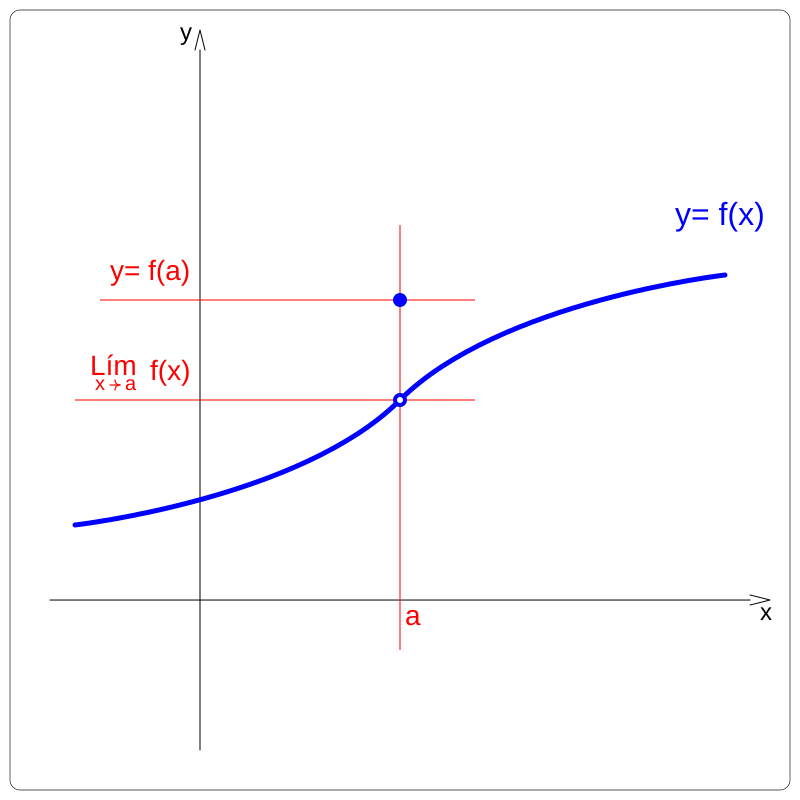
\includegraphics[scale=0.25]{img/Funs/funcion_xy_discontin_4hStg}
\caption{Ejemplo de discontinuidad evitable}
\label{fig::fun-tipos-discontinuidad}
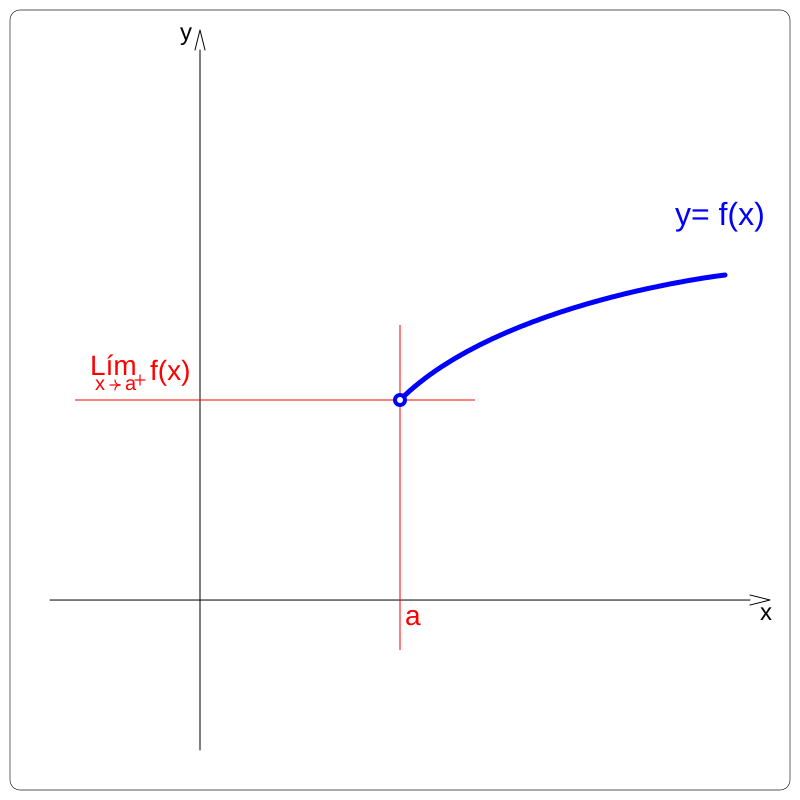
\includegraphics[scale=0.25]{img/Funs/funcion_xy_discontin_4jSGg}
\caption{Ejemplo de discontinuidad de 2ª especie}
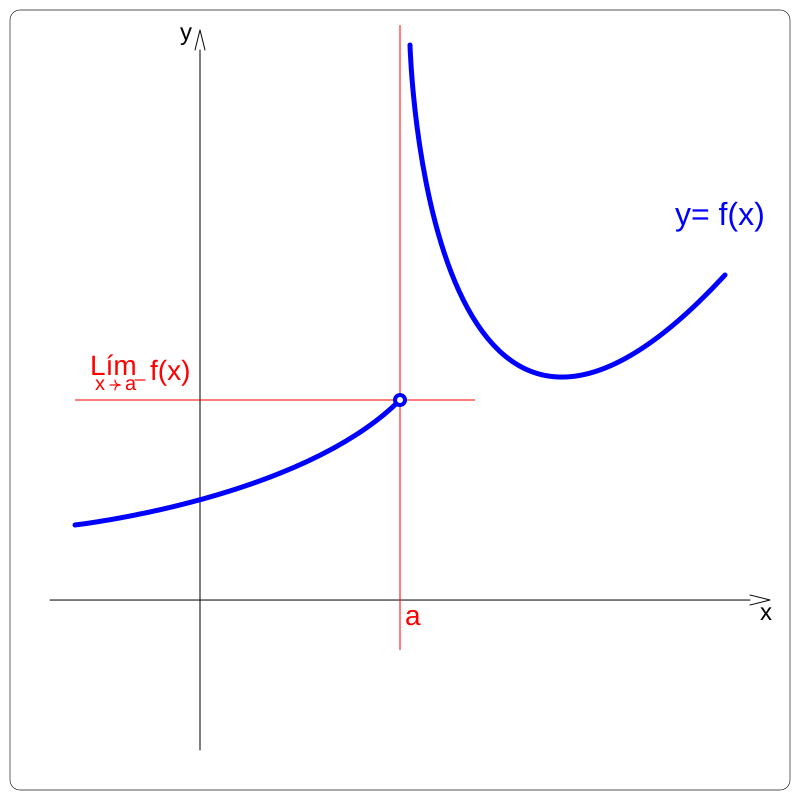
\includegraphics[scale=0.25]{img/Funs/funcion_xy_discontin_6ueR5}
\caption{Ejemplo de discontinuidad de salto infinito}
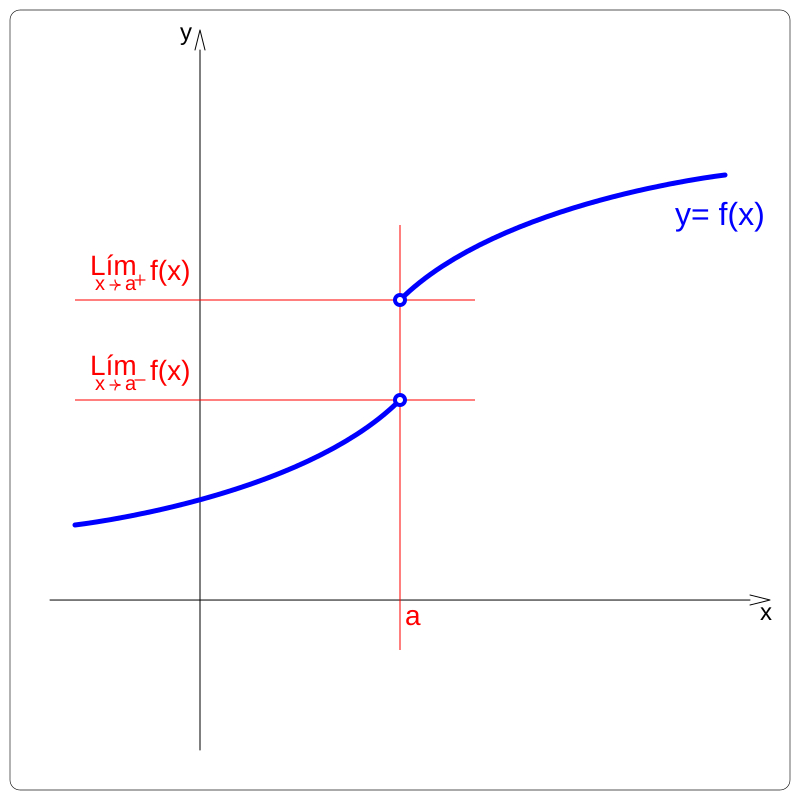
\includegraphics[scale=0.25]{img/Funs/funcion_xy_discontin_U72G2}
\caption{Ejemplo de discontinuidad de salto finito}
\end{figure}



\begin{defn}[Continuidad\IS en un intervalo abierto]

	$f(x)$ es continua en $(a,b) \dimplies \forall x\in(a,b), f(x)$ es continua.
\end{defn}


\begin{defn}[Continuidad\IS por la izquierda y/o por la derecha]
	\begin{itemize}
		\item Una función $(x)$ es continua por la derecha de $a$ si $\displaystyle\lim_{x\to a^+}f(x) = f(x)$
		\item Una función $(x)$ es continua por la izquierda de $a$ si $\displaystyle\lim_{x\to a^-}f(x) = f(x)$
	\end{itemize}
\end{defn}

\begin{defn}[Continuidad\IS en un intervalo cerrado]

$f(x)$ es continua en $[a,b] \dimplies \forall x\in[a,b],\begin{cases} f(x) \text{ es continua en } (a,b)\\
\text{Continua por la derecha de } a\\
\text{Continua por la izquierda de } b\\\end{cases}$
\end{defn}


\begin{example}
Dada $f(x) = +\sqrt{x}$.

$f(x)$ es continua en su dominio, por ser función radical. $f(x)$ continua en $(0,\infty)$.

$f(x)$ no es continua en $x=0$, pero sí es continua \textit{por la derecha} en $x=0$, ya que $\displaystyle\lim_{x\to 0^+} f(x) = 0$ en $[0,\infty)$.
\end{example}


\begin{table}[hbtp]
\begin{tabular}{|l|l|}
\hline
Funciones polinómicas & Continuas en $\real$\\\hline\hline
$f(x) = \frac{P(x)}{Q(x)}$ con $P(x),Q(x)$ polinomios& Continuas en $\real-\{x \tq Q(x)=0\}$\\\hline
$f(x) = \sqrt[n]{P(x)}$ & $\begin{cases}
n\text{ impar: continua en } \real\\\hline
n\text{ par: continua en } \{x\in\real\tq P(x) \geq 0\}\end{cases}$\\\hline
$f(x) = a^x$ con $a>0$ & Continua en $\real$\\\hline
$f(x) = \log_ax$ (con $a>0, a\neq 1$) & Continua en $\real$\\\hline
%$f(x) = \cos(x)$ y $f(x) = \sen(x)$  & Continua en $\real$\\\hline
%$f(x) = \tg(x)$   & Continua en $\real-\left\{x=\rfrac{\pi}{2}k, k\in\mathbb{Z}\right\}$\\\hline
%$f(x) = \arcsen(x)$ & Continua en su dominio.\\
%$f(x) = \arccos(x)$ & Continua en su dominio.\\
%$f(x) = \arctg(x)$ & Continua en su dominio.\\\hline
\end{tabular}
\label{tbl::ContinuidadFunElementales}
\caption{Continuidad de las funciones elementales}
\end{table}


\begin{problem}Estudia la continuidad de las siguientes funciones y clasifica sus discontinuidades

\begin{itemize}
	\item $f_1(x) = \displaystyle\frac{x^2+5x+6}{x^2+2x}$
	\item $f_2(x) = \begin{cases}\log{x+1} & x\leq -1\\x & x>1\end{cases}$
\end{itemize}
\solution
\end{problem}



\begin{theorem}[Teorema\IS de Bolzano]
Sea $\appl{f}{D}{\real}$.

\[
\left.\begin{array}{c}f(x) \text{ continua en } [a,b]\\\text{Signo}(f(a))\neq \text{Signo}(f(b))\end{array}\right\}\implies \exists c\in(a,b) \tq f(c) = 0
\]

\end{theorem}
\obs Es una condición suficiente, no necesaria. Es decir, es $\implies $. Por ejemplo, $f(x) = (x-1)^2$ corta en $x=1$, pero no cumple las condiciones.

\begin{problem} Demuestra que la ecuación $x^3-7x^2-1$ tiene al menos una solución real en el intervalo $[0,10]$.
\solution

Sea $f(x) = x^3-7x^2-1$. Se trata de demostrar que $\exists c\in[0,10]\tq f(c) = 0$. Comprobamos que cumple el teorema de Bolzano.

\[
\left\{
	\begin{array}{c}
		f(x) \text{ es continua en } [0,10] \text{ por ser polinómica}\\
		\left.\begin{array}{c}
		f(x) = -1 \\
		f(10) = 299\end{array}
		\right\}\implies Signo(f(0))\neq Signo(f(10))
	\end{array}
\right\}\implies \exists c\in(0,10)\tq f(c)=0 
\]
\end{problem}

\begin{theorem}[Teorema\IS del valor intermedio]
Sea $\appl{f}{D}{\real}$.
\[
\left.\begin{array}{c}f(x) \text{ continua en } [a,b]\\
\exists k\in\real \begin{cases}f(a)\leq k\leq f(b)\\ \text{           ó} \\f(b)\leq k \leq f(a)\end{cases}\end{array}\right\}\implies \exists c\in(a,b) \tq f(c) = k
\]
\end{theorem}

\obs Para $k=0$, el teorema del valor intermedio se convierte en teorema de Bolzano.


\begin{problem}
Demuestra que las funciones $f(x) = \log(x+10)$ y $g(x) = x$ se cortan en algún punto.
\solution

Basta considerar la función $h(x) = f(x) - g(x) = \log_5(x+10)-x$. Así, demostrar que las funciones se cortan será equivalente a demostrar que $\exists c\in\real\tq h(x)=0$. 

Esta función es continua en $\real$, por ser resta de funciones continuas en $\real$.

Buscamos $c\in\real\tq h(c)=0$. Consideramos $h(-9) = -8<0$ y $h(0)= 1 >0$.

Por el teorema de Bolzano, $\exists c\in (-9,0)\tq h(c) = 0$, por lo que podemos concluir que las funciones se cortan.
\end{problem}

%%%%%%%%%%%%%%%%%%%%%%%%%%%%%%%%%%%%%%%%%%%%%%%%%%%%%%%%%%%%%%%%%%
%%%%%%%%%%%%%%%%%%%%%%%%%%%%%%%%%%%%%%%%%%%%%%%%%%%%%%%%%%%%%%%%%%
%%%%%%%%%%%%%%%%%%%%%%%%%%%%%%%%%%%%%%%%%%%%%%%%%%%%%%%%%%%%%%%%%%
%%%%%%%%%%%%%%%%%%%%%%%%%%%%%%%%%%%%%%%%%%%%%%%%%%%%%%%%%%%%%%%%%%
%%%%%%%%%%%%%%%%%%%%%%%%%%%%%%%%%%%%%%%%%%%%%%%%%%%%%%%%%%%%%%%%%%
%%%%%%%%%%%%%%%%%%%%%%%%%%%%%%%%%%%%%%%%%%%%%%%%%%%%%%%%%%%%%%%%%%
%%%%%%%%%%%%%%%%%%%%%%%%%%%%%%%%%%%%%%%%%%%%%%%%%%%%%%%%%%%%%%%%%%
%%%%%%%%%%%%%                                    %%%%%%%%%%%%%%%%%
%%%%%%%%%%%%%                                    %%%%%%%%%%%%%%%%%
%%%%%%%%%%%%%                                    %%%%%%%%%%%%%%%%%
%%%%%%%%%%%%%                                    %%%%%%%%%%%%%%%%%
%%%%%%%%%%%%%            DERIVABILIDAD           %%%%%%%%%%%%%%%%%
%%%%%%%%%%%%%                                    %%%%%%%%%%%%%%%%%
%%%%%%%%%%%%%                                    %%%%%%%%%%%%%%%%%
%%%%%%%%%%%%%                                    %%%%%%%%%%%%%%%%%
%%%%%%%%%%%%%                                    %%%%%%%%%%%%%%%%%
%%%%%%%%%%%%%%%%%%%%%%%%%%%%%%%%%%%%%%%%%%%%%%%%%%%%%%%%%%%%%%%%%%
%%%%%%%%%%%%%%%%%%%%%%%%%%%%%%%%%%%%%%%%%%%%%%%%%%%%%%%%%%%%%%%%%%
%%%%%%%%%%%%%%%%%%%%%%%%%%%%%%%%%%%%%%%%%%%%%%%%%%%%%%%%%%%%%%%%%%
%%%%%%%%%%%%%%%%%%%%%%%%%%%%%%%%%%%%%%%%%%%%%%%%%%%%%%%%%%%%%%%%%%
%%%%%%%%%%%%%%%%%%%%%%%%%%%%%%%%%%%%%%%%%%%%%%%%%%%%%%%%%%%%%%%%%%
%%%%%%%%%%%%%%%%%%%%%%%%%%%%%%%%%%%%%%%%%%%%%%%%%%%%%%%%%%%%%%%%%%
%%%%%%%%%%%%%%%%%%%%%%%%%%%%%%%%%%%%%%%%%%%%%%%%%%%%%%%%%%%%%%%%%%

\newpage\section{Derivadas y derivabilidad}

\subsection{Introducción y repaso}
\begin{defn}[Pendiente de una recta]
Sea la recta $y=mx+n$.

Se define \textbf{pendiente de la recta}, $m=\frac{\Delta y}{\Delta x}$
\end{defn}

\begin{defn}[Derivada\IS en un punto]
Se define $f'(a)$ como la derivada de $f(x)$ en el punto $x=a$.

\[f'(a) = \lim_{x\to a}\frac{f(x)-f(a)}{x-a} \overset{(1)}{=} \lim_{h\to 0}\frac{f(a+h)-f(a)}{h}\]

$(1): h=x-a \dimplies x=a+h$

\textit{Ver \fref{fig::funinterpretacionderivadapunto}}.
\end{defn}

\begin{example}
Dada $f(x) = |x|$, calcula $f'(0)$.

\[
f(x) = \begin{cases}x&\text{ si } x>0 \\ -x & \text{ si }x\leq 0\end{cases}
\]

Calculamos:

\[
\lim_{x\to 0}\frac{f(x)-f(0)}{x-0} = \begin{cases}
\displaystyle\lim_{x\to 0^+} \frac{f(x)}{x} = \displaystyle\lim_{x\to 0^+} \frac{x}{x} = 1\\\\
\displaystyle\lim_{x\to 0^-} \frac{f(x)}{x} = \displaystyle\lim_{x\to 0^-} \frac{-x}{x} = -1
\end{cases}
\]

\label{derivEjemplo}

Los límites laterales no coinciden, por lo tanto, $\nexists \displaystyle\lim_{x\to 0}\frac{f(x)-f(a)}{x-a} \dimplies \nexists f'(a)$
\end{example}

\subsubsection{Interpretación geométrica de la derivada}

Ver \fref{fig::funinterpretacionderivadapunto}.

\begin{figure}[hbpt!]
\centering
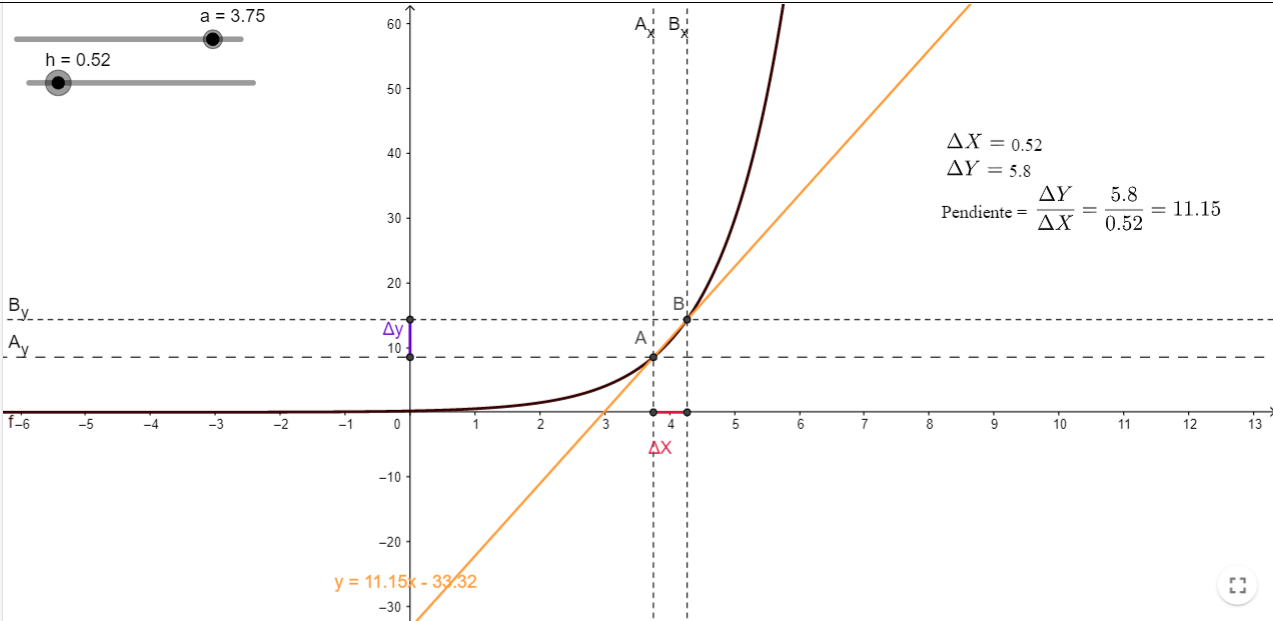
\includegraphics[scale=0.5]{img/DerivadaInterGeometrica.PNG}
\label{fig::funinterpretacionderivadapunto}
\caption{Interpretación geométrica de la derivada} Cuando $h\to0$, el punto $B$ se acercará cada vez más al punto $A$, dando lugar a la recta tangente. 
%
Para una mejor comprensión consultar la versión de Geogebra: https://www.geogebra.org/m/jwtw6mdt\#material/f52nQ7T5

\end{figure} 


\subsection{Derivabilidad}
\begin{defn}[Derivabilidad\IS en un punto]
\[f(x) \text{ derivable en } x=a\dimplies \exists f'(a)\]
\end{defn}

\begin{prop}
$f(x)$ derivable en $x=a \implies f(x)$ continua en $x=a$
\obs El recíproco no es cierto. Basta comprobar el ejemplo \ref{derivEjemplo} ($f(x) = |x|$ es continua en $x=0$, pero no derivable en $x=0$).
\end{prop}

\begin{defn}[Derivabilidad\IS en un intervalo abierto]
\[f(x) \text{ derivable en } (a,b) \dimplies \forall c\in(a,b) \exists f'(c) \]
\end{defn}

\begin{defn}[Dominio de derivabilidad]
El dominio de derivabilidad de una función $f(x)$ es el mayor conjunto en el que la función es derivable.
\end{defn}

\begin{example}
$f(x) = |x|$ no es derivable en $x=0$.

El dominio de derivabilidad de $f(x)$ es $\real-\{0\}$
\end{example}


\paragraph{Derivabilidad lateral:} De la misma manera que existía la \textit{continuidad lateral}, también podemos hablar de \textit{derivabilidad lateral}. 

\begin{defn}[Derivada lateral]
La derivada lateral de $f$ en $x=a$ por la derecha, escrita $f'(a^+)$, si existe:

\[f'(a^+) = \lim_{h\to 0^+} \frac{f(x+h)-f(x)}{h}\]

La derivada lateral de $f$ en $x=a$ por la izquierda, escrita $f'(a^-)$, si existe:

\[f'(a^-) = \lim_{h\to 0^-} \frac{f(x+h)-f(x)}{h} =  \lim_{h\to 0^+} \frac{f(x-h)-f(x)}{-h}\]

\obs Esta última igualdad se debe a que $h\to 0^-\implies h<0$. Si resulta menos confuso, puede elegirse trabajar siempre con $h>0$ y así los signos quedan explicitados.
\end{defn}

\begin{problem} Estudia la derivabilidad en $x=0$ de la función 
\label{prb::derivab1}
\[f(x) = \begin{cases} x^2+3x & \text{ si } x\leq 0\\ 3·\left(\frac{x^2+x}{x+1}\right)&\text{ si } x>0\end{cases}\]
\solution

$f(x)$ será derivable en $x=0$ si $\exists f'(0)$. Dado que $f(x)$ está definida a trozos, calculamos las derivadas laterales.

\[f'(0^-) = \lim_{h\to 0^+} \frac{f(0-h)-f(0)}{-h} = \lim_{h\to 0^-} \frac{(0-h)^2+3·(0-h)-(0^2+3·0)}{-h} = \lim_{h\to 0^-} \frac{h(h-3)}{-h} = +3\]
\[f'(0^+) = \lim_{h\to 0^+} \frac{f(0+h)-f(0)}{h} = \lim_{h\to 0^+} \frac{3·\frac{(0+h)^2+(0+h)}{0+h+1} - (0^2-3·0)}{h} = \lim_{h\to 0^+} \frac{3·\frac{h^2+h}{h+1}}{h} = \]
\[=\lim_{h\to 0^+} \frac{3·h·(h+1)}{h(h+1)} = 3 \]

\textbf{Conclusión:} Dado que  $f'(0^-) \eq f'(0^+) \implies f'(0) = 3$, por lo que la función es derivable en $x=0$.

\begin{figure}[h!]
\centering
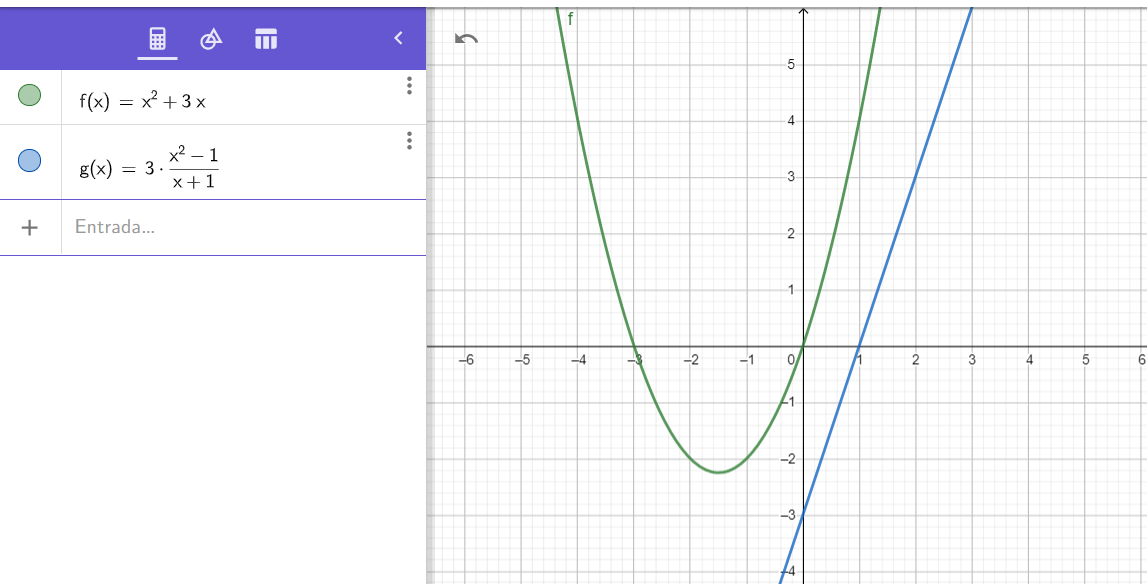
\includegraphics[scale=0.5]{img/DerivabilidadEjer1}
\label{fig::DerivabEjer1}
\caption{Representación gráfica del problema \ref{prb::derivab1}.}
Claramente la derivada en $x=0$ no puede existir, dado que la función no es continua.
\end{figure}

\obs También podríamos haber calculado la derivada lateral por la izquierda de la siguiente manera:

\[f'(0^-) = \lim_{h\to 0^-} \frac{f(0+h)-f(0)}{h} = \lim_{h\to 0^-} \frac{h^2+3·h-(0^2+3·0)}{h} = \lim_{h\to 0^-} \frac{h(h+3)}{h} = +3\]

\end{problem}


\begin{problem} Estudia la derivabilidad en $x=0$ de la función 
\label{prb::derivab1}
\[f(x) = \begin{cases} x^2+3x & \text{ si } x\leq 0\\ 3·\left(\frac{x^2-1}{x+1}\right)&\text{ si } x>0\end{cases}\]
\solution

$f(x)$ será derivable en $x=0$ si $\exists f'(0)$. Dado que $f(x)$ está definida a trozos, calculamos las derivadas laterales.

.\vspace{4cm}.
%\[f'(0^-) = \lim_{h\to 0^+} \frac{f(0-h)-f(0)}{-h} = \lim_{h\to 0^-} \frac{(0-h)^2+3·(0-h)-(0^2+3·0)}{-h} = \lim_{h\to 0^-} \frac{h(h-3)}{-h} = +3\]
%\[f'(0^+) = \lim_{h\to 0^+} \frac{f(0+h)-f(0)}{h} = \lim_{h\to 0^+} \frac{3·\frac{(0+h)^2+(0+h)}{0+h+1} - (0^2-3·0)}{h} = \lim_{h\to 0^+} \frac{3·\frac{h^2+h}{h+1}}{h} = \]
%\[=\lim_{h\to 0^+} \frac{3·h·(h+1)}{h(h+1)} = 3 \]

\textbf{Conclusión:} %Dado que  $f'(0^-) \neq f'(0^+)$,  la función no es derivable en $x=0$.

\begin{figure}[pb!]
\centering
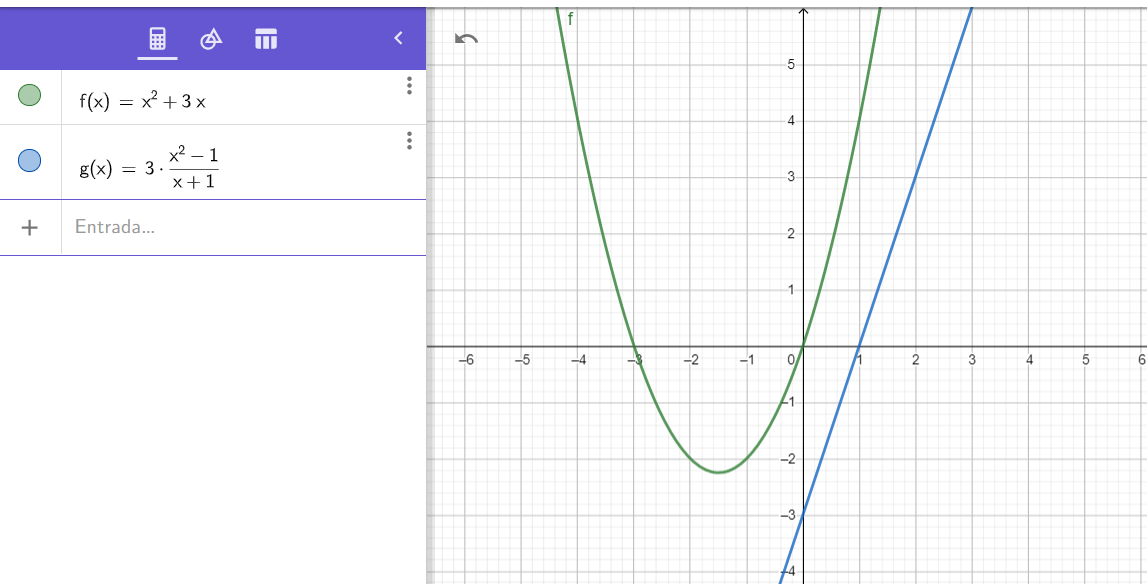
\includegraphics[scale=0.5]{img/DerivabilidadEjer1}
\label{fig::DerivabEjer1}
\caption{Representación gráfica del problema \ref{prb::derivab1}.}
Claramente la derivada en $x=0$ no puede existir, dado que la función no es continua.
\end{figure}

\obs También podríamos haber calculado la derivada lateral por la izquierda de la siguiente manera:

\[f'(0^-) = \lim_{h\to 0^-} \frac{f(0+h)-f(0)}{h} = \lim_{h\to 0^-} \frac{h^2+3·h-(0^2+3·0)}{h} = \lim_{h\to 0^-} \frac{h(h+3)}{h} = +3\]

\end{problem}

\hline

\begin{problem}
¿Es la siguiente función derivable en $x=-2,x=0,x=2$?

\[f(x) = \begin{cases}
x^2 & \text{ si } x<-2\\
-4(x+1) & \text{ si } -2<x\leq0\\
3x^2-4 & \text{ si } 0<x\leq2\\
12x+1 & \text{ si } x>2
\end{cases}\]
\solution
.\vspace{10cm}.
\end{problem}


\subsubsection{Función derivada}

\begin{defn}[Función derivada]
Dada $\appl{f}{D(f)\subset\real}{\real}$. Sea $Dv(f)$ el dominio de derivabilidad de $f$.

La función derivada denotada por $\appl{f'(x)}{Dv(f)\subset\real}{\real}$ hace corresponder a cada $a\in Dv(F)$ el valor $f'(a)$.
\end{defn}

% \begin{table}[hbp]
% \centering
% \begin{tabular}{|c|c|}\hline
% Función & Derivada\\
% \hline
% a&b\\\hline
% \end{tabular}
% \caption{Tabla de derivadas}
% \label{tbl::Derivadas}
% \end{table}

\obs Nos saltamos todas las reglas de derivación porque ya las conoces.

\obs Para estudiar la derivabilidad de una función a trozos en un punto $x=a$ puedes calcular la función derivada de cada rama y comprobar dos condiciones:
\begin{itemize}
	\item Los límites laterales en $x=a$ de esa función derivada coinciden.
	\item $f(x)$ es continua en $x=a$
\end{itemize}

\paragraph{Observación de la observación:} si estudias las derivadas laterales, no es necesario estudiar la continuidad puesto que, si la función no es continua, no será derivable. 

\textit{¿Distingues "derivadas laterales" de "límites laterales de la derivada"? Son conceptos bastante diferentes}

\begin{problem}
¿Es la siguiente función derivable en $x=-2,x=0,x=2$?

\[f(x) = \begin{cases}
x^2 & \text{ si } x<-2\\
-4(x+1) & \text{ si } -2<x\leq0\\
3x^2-4 & \text{ si } 0<x\leq2\\
12x+1 & \text{ si } x>2
\end{cases}\]
\solution

.\vspace{10cm}.

\end{problem}

\begin{problem}
Dada la función $f(x)$, calcula $a,b,c\in\real$ para que la función sea derivable en $x=1$, sabiendo que $f(0) = f(4)$.

\[
f(x) = 
\begin{cases}
	x^2+ax+b&\text{ si } x<1\\
	cx & \text{ si } x\geq 1
\end{cases}
\]
\solution

Solución: $a=-\rfrac{7}{4}; b=1; c=\rfrac{1}{4}$

%\begin{figure}[h!]
%\centering
%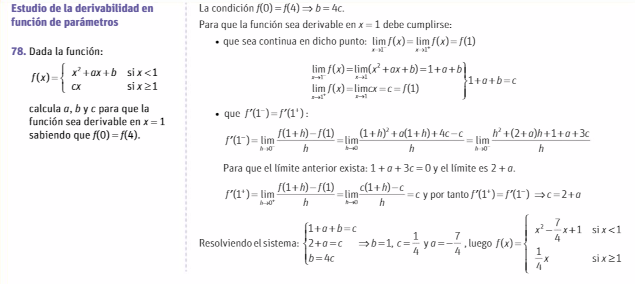
\includegraphics[scale=1.1]{img/DerivabilidadEjer5678.png}
%\label{ejercicioDerivabilidad}
%\caption{Ejercicio sacado del libro de SM}
%\end{figure}

\end{problem}



\subsection{Aplicaciones de la derivada}

\subsubsection{Recta tangente y recta normal}

\paragraph{Ecuación de la recta tangente:} Utilizando la ecuación de la recta punto-pendiente y la interpretación gráfica de la derivada (ver \ref{fig::funinterpretacionderivadapunto}), se obtiene fácilmente la siguiente ecuación:

\begin{mdframed}
	\begin{equation}
		\label{eq::rectatangente}
		\text{Recta tangente a }f(x)\text{ en }x_0 \to y-f(x_0) = f'(x_0)·(x-x_0)
	\end{equation}
\end{mdframed}

\begin{problem}
Calcula las rectas tangente a la gráfica de $f(x) = x^3+2x$ en $x=1$.
\solution

Aplicamos: $\text{Recta tangente a }f(x)\text{ en }x_0 \to y-f(x_0) = f'(x_0)·(x-x_0)$

Para ello, calculamos:
\begin{itemize}
	\item $f(x_0)=$
	\item $f'(x)$
	\subitem $f'(x_0)$
\end{itemize}
Sustituyendo en la ecuación, obtenemos:
.\vspace{2cm}.
\end{problem}

\begin{problem}
Demuestra que la recta $y=-x$ es tangente a la curva dada por la ecuación: $y=x^3+6x^2+8x$
\solution

Consideramos $f(x) = x^3-6x^2+8x \to f'(x) = 3x^2-12x+8$.

Buscamos $c\in\real\tq f'(c) = -1$.

\[
	3c^2+12c+8=-1 \dimplies \begin{cases}c_1 = 1\\c_2=3\end{cases}
\]

Los posibles puntos de tangencia son $P_1(c_1,f(c_1)) = (1,3)$ y $P_2(c_2,f(c_2)) = (3,-3)$.

Es necesario comprobar que dichos puntos son realmente de tangencia, es decir, que pertenecen a la recta y a la gráfica.

\[P_1: 3\neq -1 \implies \text{ no pertenece a la recta}\]
\[P_2: -3\eq -3 \implies \text{ sí pertenece a la recta}\]

\textbf{Conclusión: } El punto de tangencia de la recta $y=-x$ a la gráfica $f(x) = x^3-6x^2+8x$ es $P_2(3,-3)$
\end{problem}

\paragraph{Ecuación de la recta normal:} Dos rectas dadas, en 2 dimensiones, $r: y=m_rx+n_r\quad;\quad s:y=m_sx+n_s$ son perpendiculares si y sólo si $m_r·m_s = -1 \dimplies m_s = \rfrac{-1}{m_r}$.
%
Aplicando este resultado a la fórmula de la recta tangente anterior, tenemos:


\begin{mdframed}
	\begin{equation}
		\label{eq::rectatangente}
		\text{Recta normal a }f(x)\text{ en }x_0 \to y-f(x_0) = \rfrac{-1}{f'(x_0)}·(x-x_0)
	\end{equation}
\end{mdframed}

\begin{problem}
Calcula las rectas tangente a la gráfica de $f(x) = x^3+2x$ en $x=1$.
\solution

Aplicamos: $\text{Recta normal a }f(x)\text{ en }x_0 \to y-f(x_0) = \rfrac{-1}{f'(x_0)}·(x-x_0)$

Para ello, calculamos:
\begin{itemize}
	\item $f(x_0)=$
	\item $f'(x)$
	\subitem $f'(x_0)$
\end{itemize}
Sustituyendo en la ecuación, obtenemos:
.\vspace{2cm}.
\end{problem}



\subsubsection{Teoremas de derivabilidad}

(Ver documento aparte)

%\begin{theorem}[Teorema\IS de Rolle]
%\[
%\left.
%	\begin{array}{c}
%		f(x)\text{ continua en } [a,b]\\
%		f(x)\text{ derivable en } (a,b)\\
%		f(a)=f(b)
%	\end{array}
%\right\}\implies \exists c\in(a,b)\tq f'(c)=0
%\]
%\end{theorem}
%\obs ¿Puede haber más de un punto? ¡Claro que sí! Basta pensar en una función horizontal.
%
\begin{problem}
% Página 66.1
Sea $f(x) = 2x^5+x+a$.  Demuestra que $\exists!c\in\real\tq f(c)=0$
\solution
Por el teorema de Bolzano, hay al menos una raíz real.

\ul{Veamos que es única.} Si hubiera otra raíz real, $d$, tendríamos $f(c) = f(d)$ en una función continua en $[c,d]\subset\real$ y derivable en $(c,d)\subset\real$ por ser una función polinómica.
%
Así, se puede aplicar el teorema de Rolle, argumentando que $\exists c\in\real\tq f'(c) = 0$, pero $f'(x) = 10x^4+1 \neq 0 \;\forall x\in\real$.

\textbf{Conclusión: } dado que $f(x)$ cumple todas las hipótesis del teorema de Rolle, debemos concluir necesariamente que no hay otra raíz real $d$\footnote{Sino, el teorema fallaría y eso no es posible.}. 
\end{problem}


%\begin{theorem}[Teorema\IS del valor medio]
%\[
%\left.
%	\begin{array}{c}
%		f(x)\text{ continua en } [a,b]\\
%		f(x)\text{ derivable en } (a,b)\\
%	\end{array}
%\right\}\implies \exists c\in(a,b)\tq f'(c)=\frac{f(b)-f(a)}{b-a}
%\]
%
%\obs El teorema de Rolle es un caso particular de este teorema que se da cuando $f(a) = f(b)$
%\end{theorem}
%\obs ¿Puede haber más de un punto? ¡Claro que sí!

\begin{problem}
Considera la función $f(x) = x·e^{-x^2}$.

Calcula el valor del parámetro real $a$ para el que se puede aplicar el teorema de Rolle en el intervalo $[0,1]$ a la función $g(x) = f(x) + ax$
\solution

\[g(x) = x·e^{-x^2} + ax = x·\left(a+e^{-x^2}\right)\]

Las hipótesis del teorema de Rolle son:

\[
\left.
	\begin{array}{l}
		g(x)\text{ continua en } [0,1] \to \text{ En este caso sí por ser suma de función polinómica y exponencial}\\
		g(x)\text{ derivable en } (0,1) \to \text{ En este caso sí por ser suma de función polinómica y exponencial}\\
		g(a)=g(b) 
	\end{array}
\right\}
\]

Necesitamos que $g(0) = g(1)$. 

\[0·\left(a+e^{-0^2}\right) = 1·\left(a+e^{-1^2}\right) \dimplies 0 = a+e^{-1} \dimplies a=-e^{-1}\]

\obs Este problema salió en las noticias de 2019 porque se preguntó en la EVAU de valencia y los alumnos se enfadaron mucho.
\end{problem}

\begin{problem}

\ppart[17.2-MadA] Estudia la derivabilidad en $x=0$ de $f(x) = \begin{cases}\displaystyle x·e^{2x} &\mbox{ si } x<0\\ \displaystyle\frac{\ln(x+1)}{x+1}&\mbox{ si } x\geq 0\end{cases}$ en $x=0$. 
\ppart[16.1-MadB] Determina el polinomio $f(x)$, sabiendo que $\forall x\in\real f'''(x) = 12$ y además verifica $f(1) = 3; f'(1) = 1; f''(1) = 4$.
\ppart[16.1-MadB] Estudie la continuidad y la derivabilidad en $x=0$ y en $x=1$ de $f(x) = \begin{cases} 0& \text{ si } x\leq 0\\|x\ln(x)&\text{ si} x>0\end{cases}$
\solution
\end{problem}

\subsubsection{Regla de L'Hôpital}
(Ver documento aparte)
\subsubsection{Monotonía}
\subsubsection{La segunda derivada: Curvatura}
\subsubsection{Optimización}
\section{Análisis sistemático de una función}
\section{Integrales}
\subsection{Primitivas}
\subsection{Cálculo de áreas de recintos cerrados}